\documentclass[11pt, oneside]{article}   	% use "amsart" instead of "article" for AMSLaTeX format
\usepackage{geometry}                		% See geometry.pdf to learn the layout options. There are lots.
\geometry{letterpaper}                   		% ... or a4paper or a5paper or ... 
%\geometry{landscape}                		% Activate for for rotated page geometry
%\usepackage[parfill]{parskip}    		% Activate to begin paragraphs with an empty line rather than an indent
\usepackage{graphicx}				% Use pdf, png, jpg, or eps� with pdflatex; use eps in DVI mode
								% TeX will automatically convert eps --> pdf in pdflatex		
\usepackage{amssymb}
\usepackage{amsmath}
\usepackage{parskip}
\usepackage{color}
\usepackage{url}

\title{Differentiating under the integral sign}
%\author{The Author}
%\section{}
% \subsection*{R code}
\date{}							% Activate to display a given date or no date

\graphicspath{{/Users/telliott_admin/Dropbox/Tex/png/}}

% \begin{center} 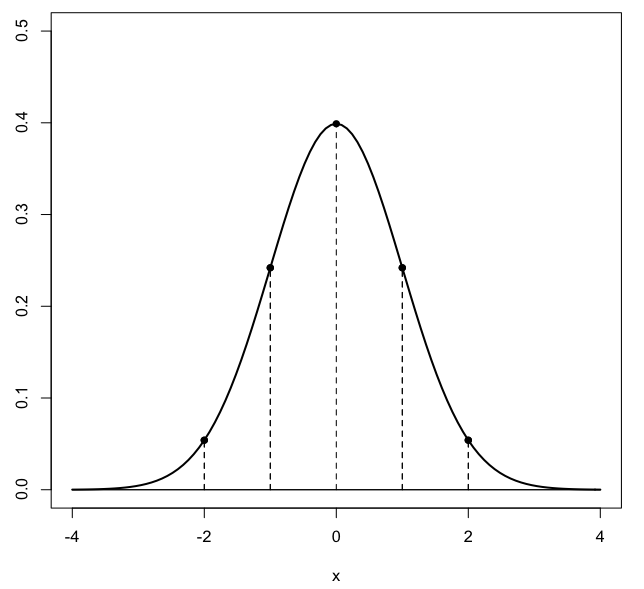
\includegraphics [scale=0.4] {gauss3.png} \end{center}
% \begin{bmatrix} a  &  b \\ c  &  d \end{bmatrix}
% \bigg |_

\begin{document}
\maketitle
\large

In \emph{Surely you're joking, Mr. Feynman}, Richard Feynman says the following:

I had learned to do integrals by various methods shown in a book that my high school physics teacher Mr. Bader had given me. [It] showed how to differentiate parameters under the integral sign --- it's a certain operation. It turns out that's not taught very much in the universities; they don't emphasize it. But I caught on how to use that method, and I used that one damn tool again and again. [If] guys at MIT or Princeton had trouble doing a certain integral, [then] I come along and try differentiating under the integral sign, and often it worked. So I got a great reputation for doing integrals, only because my box of tools was different from everybody else's, and they had tried all their tools on it before giving the problem to me.

\subsection*{Introduction}

Suppose $f(x,t)$ is a function of $x$ and $t$ (defined) on the rectangle $R$, where $R = [a,b] \times [c,d]$.  That is, the bounds of the rectangle are $a \le x \le b$ and $c \le t \le  d$.

Suppose also that $\partial f/\partial t$ is continuous on $R$.

Then, \textbf{Leibnitz's Rule} says that

\[ \frac{d}{dt} \ \int_a^b f(x,t) \ dx =  \int_a^b g(x,t) \ dx \]
where
\[ g(x,t) = \frac{\partial}{\partial t}  f(x,t)\]
We'll look at some uses of this rule in the sections below.

\subsection*{improper integral}
Let's start by recalling how to evaluate the improper integral
\[ \int_0^{\infty} e^{-x} \ dx \]

This is accomplished by substituting a finite upper bound $b$ for $\infty$ and doing the integral, then seeing what happens in the limit as $b \rightarrow \infty$.
\[ \int_0^b e^{-x} \ dx = -e^{-x} \ \bigg |_0^b =  -\frac{1}{e^{x}} \ \bigg |_0^b = \frac{1}{e^0} - \frac{1}{e^b} \]
In the limit, the second term becomes zero so the integral is just equal to 1:
\[ \int_0^{\infty} e^{-x} \ dx  = 1 \]

Now, suppose we have
\[ \int_0^{\infty} e^{-tx} \ dx \]
where $t$ does not depend on $x$.
We know that
\[ \int e^{ax} \ dx = \frac{1}{a} \ e^{ax} \]
(easily verified by differentiating), and thus
\[ \int_0^b e^{-tx} \ dx = -\frac{1}{t} \ [ \ e^{-tx} \ \bigg |_0^b \ ] \]
\[ =  -\frac{1}{t} \ [ \  \frac{1}{e^{tx}} \ \bigg |_0^b \ ] \ \]
\[ = \frac{1}{t} \ [ \ \frac{1}{e^0} - \frac{1}{e^{bt}} \ ]  \]
In the limit as $b \rightarrow \infty$, the term in brackets becomes $ [ \ 1-0 \ ] \ = 1$ so the integral is just $1/t$:
\[ \int_0^{\infty} e^{-tx} \ dx  = \frac{1}{t} \]

\subsection*{factorial}

Now, apply Liebnitz's rule!
\[ \frac{d}{dt} \ \int_0^{\infty} e^{-tx} \ dx = \int_0^{\infty} \frac{\partial}{\partial t} \  e^{-tx} \ dx \]
Substitute the result from above on the left-hand side:
\[ \frac{d}{dt} \ \frac{1}{t} = - \frac{1}{t^2} = - t^{-2} \]
Differentiate \emph{with respect to} $t$ on the right-hand side:
\[ - t^{-2} = \int_0^{\infty} -x \  e^{-tx} \ dx \]
Rearranging:
\[ \int_0^{\infty} x e^{-tx} \ dx = t^{-2} \]

This can be continued indefinitely:
\[ \int_0^{\infty} x^2 e^{-tx} \ dx = 2 t^{-3} \]
Here we have simply repeated the differentiation with respect to $t$ on both sides, while canceling the minus signs.

And again:
\[ \int_0^{\infty} x^3 e^{-tx} \ dx = (2 \cdot 3) \ t^{-4} \]
\[ \int_0^{\infty} x^n e^{-tx} \ dx = n! \  t^{-(n+1)} \]
Finally, just let $t=1$:
\[  \int_0^{\infty} x^n e^{-x} \ dx = n!  \]

This is Euler's factorial integral.  It is often written with $t$ switched in for $x$ and $x$ for $n$:
\[  \int_0^{\infty} t^x e^{-t} \ dt = x!  \]
and the Gamma ($\Gamma$) function is defined
\[ \Gamma(x+1) = x! =  \int_0^{\infty} t^x e^{-t} \ dt \]
equivalently
\[ \Gamma(n) = (n-1)! =  \int_0^{\infty} t^{n-1} e^{-t} \ dt \]

\subsection*{integration by parts}

Euler's factorial integral can also be derived using integration by parts starting from 
\[ \int_0^{\infty} e^{-x} \ dx  = 1 \]
which is where we started, above.  Now, suppose we have
\[ \int_0^{\infty} x^n e^{-x} \ dx  \]
with $n=1$
\[ \int_0^{\infty} x e^{-x} \ dx  \]
let 
\[ u = x, \ \ \ du = dx \]
\[ dv = e^{-x} \ dx, \ \ \ v = -e^{-x} \]
so the integral is
\[ = - x e^{-x} \bigg |_0^{\infty} - \int_0^{\infty} -e^{-x} \ dx \]

The second term is our previous result.  At the lower bound, the first term is zero.  So we must evaluate:
\[ \lim_{x \rightarrow \infty} -x e^{-x} \]
\[ = \lim_{x \rightarrow \infty} \frac{-x}{e^{x}} = \frac{- \infty}{\infty} \]
Use L'Hopital's Rule and differentiate:
\[ = \lim_{x \rightarrow \infty} \frac{-1}{e^{x}} = \frac{-1}{\infty} = 0 \]
Therefore, the entire first term is zero and the result of the integral is just 1.
\[ \int_0^{\infty} x e^{-x} \ dx  = 1 \]

The general case is:
\[ \int_0^{\infty} x^n e^{-x} \ dx \]
As before, we use integration by parts:
\[ u = x^n, \ \ \ du = n x^{n-1} \ dx \]
\[ dv =  e^{-x} \ dx, \ \ \ v = -e^{-x} \]
    
So the integral is:
\[ = -x^n e^{-x} + n \int x^{n-1} e^{-x} \ dx \]
The first term is equal to zero by the analysis we did above.  We need to apply L'Hopital's rule repeatedly ($n$ times), and eventually find that the result is zero at the upper bound as well as the lower bound.

The second term is $n$ times the original integral, but with $n-1$ substituted for $n$.  Recalling that we had $f(0) = f(1) = 1$, we find that:
\[ \int_0^{\infty} x^n e^{-x} \ dx = n! \]

\subsection*{proof}
The proof of Leibnitz's Rule is pretty straightforward, if we assume that the order of integration in an iterated integral doesn't matter (Fubini's Theorem):

\[ \int_{y=c}^{y=d} \ \int_{x=a}^{x=b} g(x,y) \ dx \ dy = \int_{x=a}^{x=b} \  \int_{y=c}^{y=d}  g(x,y) \ dy \ dx \]

(see wikipedia for examples of when it does matter).

I've written the equation in terms of $x$ and $y$ because that's how it is in the original:

\url{http://math.hawaii.edu/~rharron/teaching/MAT203/LeibnizRule.pdf}

Suppose we choose for our function the partial derivative of another function $f(x,y)$
\[ g(x,y) = \frac{\partial f}{\partial y} \]
and that we take the derivative with respect to $y$ of both sides:

\[ \frac{d}{dy} \ \int_c^d \ \int_a^b \frac{\partial f}{\partial y} \ dx \ dy =   \frac{d}{dy} \ \int_a^b \  \int_c^d  \frac{\partial f}{\partial y} \ dy \ dx \]
Using one version of the fundamental theorem of calculus, namely:
\[ \frac{d}{dt} \ \int_a^t f(x) \ dx = f(t) \]
the left-hand side of our equality
\[ \frac{d}{dy} \ \int_c^d \ \int_a^b \frac{\partial f}{\partial y} \ dx \ dy \]
becomes:
\[ = \int_a^b \frac{\partial f}{\partial y} \ dx \]

Using the other version of the FTC
\[ \int_a^b F'(x) \ dx = F(b) - F(a) \]
the right-hand side
\[ \frac{d}{dy} \ \int_{x=a}^{x=b} \  \int_{y=c}^{y=d}  g(x,y) \ dy \ dx \]
becomes:
\[ = \frac{d}{dy} \ \int_a^b \ [ \  f(x,y) - f(x,c) \ ] \ dx \]
but $f(x,c)$ is not a function of $y$ so the partial derivative is just zero for the second term and we have:
\[ = \frac{d}{dy} \ \int_a^b \  f(x,y)  \ dx \]
Putting the two sides together:
\[  \int_a^b \frac{\partial f}{\partial y} \ dx = \frac{d}{dy} \ \int_a^b \  f(x,y)  \ dx \]
which is what we wanted to prove.

I am a little shaky on both these steps but I include them based on the source.

\subsection*{Gaussian}
Shankar uses as an example a series of functions related to the Gaussian
\[ I_0(a) = \int_0^{\infty} e^{-ax^2} \ dx \]
\[ I_1(a) = \int_0^{\infty} e^{-ax^2} \ x \ dx \]
and so on.  The notation $I(a)$ indicates that we will eventually view these guys as a function of the parameter $a$.

The first one is (one-half) the Gaussian integral and we will just assume the answer here:
\[ I_0(a) = \int_0^{\infty} e^{-ax^2} \ dx = \frac{1}{2} \ \sqrt{\frac{\pi}{a}} = \frac{1}{2} \ \sqrt{\pi} a^{-1/2}  \]

The second is straightforward to evaluate since we have the derivative of what's in the exponent:
\[ I_1(a) = \int_0^{\infty} e^{-ax^2} \ x \ dx = -\frac{1}{2a} \ [ e^{-ax^2} \  ] \ \bigg |_0^{\infty} \]
\[ = -\frac{1}{2a} \ (-1) = \frac{1}{2a} \]
After that (with higher powers of $x$) it's not so easy.

What we're going to do is start from $I_0(a)$ and differentiate with respect to $a$, using the rule from above.  We will have:
\[ \int_0^{\infty} \frac{\partial}{\partial a} \ e^{-ax^2} \ dx = \frac{d}{da} \  \frac{1}{2} \ \sqrt{\pi} a^{-1/2} \]
\[ \int_0^{\infty} \ e^{-ax^2} \ (-x^2) \ dx = -\frac{1}{4} \ \sqrt{\pi} a^{-3/2} \]
\[ I_2(a) = \int_0^{\infty} \ e^{-ax^2} \ x^2 \ dx = \frac{1}{4} \ \sqrt{\pi} a^{-3/2} \]
\[ I_4(a) = \int_0^{\infty} \ e^{-ax^2} \ x^4 \ dx = \frac{3}{8} \ \sqrt{\pi} a^{-5/2} \]

and so on.  For the odd functions do this:
\[ I_1(a) = \int_0^{\infty} e^{-ax^2} \ x \ dx = \frac{1}{2a} \]
\[ \int_0^{\infty} \frac{\partial}{\partial a} \ e^{-ax^2} \ x \ dx = \frac{d}{da} \ \frac{1}{2a} \]
\[ - \int_0^{\infty} \ e^{-ax^2} \ x^3 \ dx = - \frac{1}{2a^2} \]
\[ I_3(a) = \int_0^{\infty} \ e^{-ax^2} \ x^3 \ dx = \frac{1}{2a^2} \]

Thus we can solve the whole series of integrals of the form:
\[ I_n(a) = \int_0^{\infty} e^{-ax^2} \ x^n\ dx \]


\subsection*{$tan^{-1}$}
Another one is the integral which yields the inverse tangent:
\[ \int_0^{\infty} \frac{1}{1 + x^2} \ dx \]
\[ = \tan^{-1} x \ \bigg |_0^{\infty} = \frac{\pi}{2} - 0 \]
\[ =  \frac{\pi}{2} \]
It's easy to solve this with a trig substitution:
\[ x = \tan \theta \]
\[ dx = \sec^2 \theta \ d \theta \]
\[ \frac{1}{1 + x^2} = \cos^2 \theta \]
The integral is just
\[ \int d \theta = \theta = \tan^{-1} x \]

Suppose instead that we have
\[ \int_0^{\infty} \frac{1}{a^2 + x^2} \ dx \]
One way to solve this is to scale $x$:
\[ x = au, \ \ \ dx = a \ du \]
Then
\[ \int_0^{\infty} \frac{1}{a^2 + x^2} \ dx = a \int_0^{\infty} \frac{1}{a^2 + a^2u^2} \ du \]
\[ = a \int_0^{\infty} \frac{1}{a^2} \ \frac{1}{1 + u^2} \ du \]
\[ = \frac{1}{a} \int_0^{\infty} \ \frac{1}{1 + u^2} \ du \]
\[ = \frac{1}{a} \tan^{-1} u \ \bigg |_0^{\infty} = \frac{\pi}{2a} \]

So, start with that one and differentiate:
\[ \int_0^{\infty} \frac{\partial}{\partial a} \ \frac{1}{a^2 + x^2} \ dx = \frac{d}{da} \ \frac{\pi}{2a} \]
\[ - 2a \int_0^{\infty} \frac{1}{(a^2 + x^2)^2} \ dx = - \frac{\pi}{2a^2} \]
\[ \int_0^{\infty} \frac{1}{(a^2 + x^2)^2} \ dx = \frac{\pi}{4a^3} \]

\end{document}  